\chapter{Notational Conventions and Preliminaries}
\label{ch-conventions}
This book is a sequel to
my book entitled \qt{Bayesuvius}
(see Ref.\cite{bayesuvius}). 
For consistency, 
I have tried to follow in this book the 
same notational conventions
used in the prior book.
If any notation is not defined in this book,
check in the prior book. It might be
defined there.  

\section{Set notation}

The number of elements in any set $S$ is denoted by $|S|$.

$\ZZ$ = integers

$\ZZ_{>0}$ = positive integers

$\ZZ_{[a,b]} = a, a+1, \ldots, b$
for some integers $a, b$ such that $a\leq b$

$\RR$ = reals

$\CC$= complex numbers

$\CC^{n\times m}$ = $n\times m$ matrices of complex numbers

\section{Group}

A {\bf group}
$\calg$
is a set of elements
with a multiplication map $\calg\times \calg
\rarrow \calg$
such that


\begin{enumerate}
\item 
the multiplication is {\bf associative
}; i.e., 

\beq
(ab)c = a(bc)
\eeq
for $a,b,c\in\calg$.

\item
there exists an {\bf identity element}
$e\in \calg$
such that 

\beq
ea=ae=a
\eeq
for all $a\in \calg$

\item
for any $g\in\calg$,
there exists an {\bf inverse} $a^{-1}\in \calg$ such that

\beq
aa^{-1}=a^{-1}a=e
\eeq
\end{enumerate}

$|\calg|$ (i.e., number of
elements in $\calg$)
is called the {\bf order}
of the group.

If multiplication is
{\bf commutative}
(i.e., $ab=ba$ for all $a,b\in\calg$),
the group is said to be {\bf abelian}.

A {\bf subgroup} $\calh$ 
of $\calg$
is a subset of $\calg$
($\calh \subset \calg$)
which is also a group.
It's easy to show that any $\calh\subset \calg$ is a group if it
contains the identity
and is {\bf closed 
under multiplication} (i.e., $ab\in \calh$ for all $a,b\in \calh$) 



\section{Group  Representation}

A {\bf group representation} (rep)
of a group $\calg$
is a map $\phi: \calg\rarrow \CC^{n\times n}$\footnote{More generally, the $\CC^{n\times n}$ can be replaced by $\RR^{n\times n}$ or by $\FF^{n\times n}$ for any field $\FF$} such that

\beq
\phi(a)\phi(b)=
\phi(ab),
\quad \phi(e) = I
\eeq
where $e$ is the
identity of the group
and $I$ 
is the identity matrix.
Such a map is called a {\bf homomorphism}
(because it preserves an operation).
The map $\phi$ 
partitions $\calg$
into disjoints subsets (equivalence classes),
such that all elements of $\calg$ in each disjoint subset 
are represented by the same matrix.

One  way to specify a representation is
to give the effect of each group element $a\in \calg$ on a basis of vectors $\{\ket{1}, \ket{2}, \dots, \ket{n}\}$.


\beq
\phi (a)\ket{i}= \sum_j M_{ij}\ket{j}
\implies \av{i|\phi(a)|j} = M_{ij}
\eeq

If the map $\phi$
is 1-1, onto, we call it a {\bf faithful representation} 

The {\bf trivial representation} 
represents all $g\in \calg$
by  $diag(1,1, \dots, 1)$.
It's dimension is $d_\lam=0$.
It's not a faithful rep.

A {\bf singlet representation}
represents all
$g\in \calg$
by  $ z(g) diag(1,1, \dots, 1)$
for some $z(g)\in\CC$.
For the singlet rep, $\av{i|\phi(a)|j}=z(g)
\delta(i,j)$.
It's dimension is $d_\lam=1$.
The projection operator
$\delta_a^b \delta_c^d$
when acting on $G\indices{_c^d}$
gives a $ z(G) diag(1,1, \dots, 1)$
where $z(G)=\tr(G)$, so it
projects to a singlet rep.



When a group is 
defined using matrices, those
matrices are called the {\bf defining representation} (defrep). For example,
the group
of {\bf General Linear Transformations}
is defined by

\beq
GL(n, \CC)=
\{M\in \CC^{n\times n}: \det{M}\neq 0\}
\eeq

The {\bf adjoint representation} (adjrep)
is defined in terms of the structure constants
of the Lie Algebra. If the Lie Algebra satisfies
$[T^i, T^j]= if_{ijk}T^k$,
then the adjrep is given by the matrices 
with $i,j$ entries $M^k_{ij}=-if\indices{^k_i_j}$.
Let  $\ket{x} = x_i \ket{T^i}$.
Then

\beq
[\ket{x}, \cdot]\ket{T^j}   = 
\ket{[x, T^j]}= i x_if_{ijk}\ket{T^k} \implies
\bra{T^k}[\ket{x}, \cdot]\ket{T^j}= 
i x_i f_{ijk}
\eeq


{\bf Irreducible representations} (irreps)
are defined in Ch. \ref{ch-reducibility}

The {\bf fundamental representation} (funrep)
is defined as the smallest irrep.. 
The defrep equals the funrep for
$SU(n), SO(n), SP(n)$, but not for $E_8$.



\section{Group Theory References}
Much of this book
deals with Group Theory (GT).


GT is a vast subject. Who would have thought
that the simple definition of 
a group would generate so many elegant, highly applicable and useful results and
consequences.

GT books by mathematicians are very
different from GT
books by physicists,
even though, of course,
they agree on the definitions. 
Mathematicians
are, as to be expected, more rigorous and abstract. But it goes much further than that. Physicists are much
more interested in applications
to physical systems,
especially Quantum Mechanics (QM).
Soon after QM was invented,
it was realized that Linear Algebra (LA) and GT  (especially Group Representation Theory,
which combines GT and LA)
are extremely
relevant and useful in QM.
Hermann Weyl,
Eugene Wigner, Hans Bethe, Linus Pauling, etc.
combined QM and GT to understand the spectra and chemistry of atoms and molecules,
and later GT was heavily used in Quantum Field Theory and Particle Physics to devise 
the Standard Model. Condensed Matter physicists have also used it to understand crystalline solids and to devise quasi particles that can be detected in the lab. 

My PhD is in physics
so in this book I cover 
GT topics that are  mainly of interests to
physicists and engineers. Furthermore,
I am nowhere as abstract and
rigorous as mathematicians 
usually are.

My favorite books about GT 
for physicists are the Elliott \& Dawber's (ED)
2 volume series Ref. \cite{eli-daw-book}
and Predrag Cvitanovic's Birdtracks book
Ref.\cite{birdtracks-book}. I highly
recommend both of these references. I think
both of them are excellent.

The Birdtracks book explains key 
concepts in GT representation theory
using network diagrams 
(Cvitanovic calls 
such diagrams birdtracks) whereas the ED book doesn't use that type of diagram. Many people don't use birdtracks either, they only use algebra.
But since this is a book
about visualization using network diagrams (quantum 
bnets), we use birdtracks.
In fact, many
of the chapters in this
book were heavily influenced 
by Ref.\cite{birdtracks-book}
by Cvitanovic. I hope he doesn't mind. I really love his  book.

\section{Vector Space and Algebra over a field $\FF$}
\label{sec-algebra-over-f}

A vector  space
(a.k.a. linear space)  $\calv$
is defined as a set endowed with
two operations: vector addition $+:\calv\times\calv\rarrow \calv$,
and scalar multiplication $\FF\times\calv\rarrow \calv$,
such that

\begin{itemize}
\item $\calv$ is an abelian group under $+$
with identity $0$ and inverse of $x\in\calv$ equal to $-x\in\calv$

\item
For $\alp, \beta\in\FF$ and
$x,y\in\calv$
\beqa
\alp(x+y) &=& \alp x + \alp y
\\
(\alp +\beta)x &=& \alp x + \beta x
\\
\alp(\beta x)
&=&
(\alp\beta)x
\\
1x &=& x
\\
0x &=& 0
\eeqa
\end{itemize}
 In this book, we will always use either $\CC$ or $\RR$ for $\FF$. Both 
 of these fields are infinite but some fields are finite.


An {\bf algebra} $\cala$ is a
vector space  
which, 
besides being endowed with vector addition
and scalar multiplication
as all vector spaces are,
it has
a {\bf bilinear vector product}.
A bilinear vector product is a product that is linear on both sides; i.e., 

\beq
(\alp x + \beta y)\cdot z =
\alp x\cdot z +
\beta y\cdot z
\eeq
and 
\beq
z\cdot(\alp x + \beta y)=
\alp z \cdot x +
\beta z\cdot y
\eeq
for $x,y, z\in \cala$ and 
$\alp, \beta\in\CC$.
The cross product (but not the dot product)
for vectors in $\RR^3$,
the multiplication of 2 complex numbers, the product or commutator of 2
square matrices, are all good examples of
bilinear vector products.

Let $B = \{\tau_i: i=1, 2, \ldots, r\}$
be a basis for the vector space $\cala$. 
Then note that
$B$ is closed under vector multiplication. 

\beq
\tau_i\cdot \tau_j=
\sum_k c\indices{_{ij}^k} \tau_k
\eeq
where $c\indices{_{ij}^k}\in\CC$.
The $c\indices{_{ij}^k}$ are called 
{\bf structure constants} of $B$.
In Dirac notation

\beq
\tau_i\ket{\tau_j}=
\ket{\tau_i \cdot \tau_j}=
\sum_k c\indices{_i_j^k}\ket{\tau_k}
\eeq

\beq
\av{\tau_k|\tau_i|\tau_j}= c\indices{_i_j^k}
\eeq

An {\bf associative algebra} satisfies 
$(x\cdot y)\cdot z = x\cdot(y\cdot z)$ for
$x,y,z\in \cala$.
\begin{itemize}
\item Not associative: cross product for vectors in  $\RR^3$.
\item Associative:
the product or commutator of 2  square matrices and the product of complex numbers
\end{itemize}

\section{Tensors}
\label{sec-tensors}
Let 

$(x_a)=(x_1, x_2, \ldots, x_n) = x^{:n}\in V^n=\CC^{n\times 1}$

Reverse of vector $rev(x_1, x_2, \ldots, x_n)=
(x_n, x_{n-1},
\ldots, x_1)$

$y^b = \sum_a g^{ba} x_a$

$(y^b)=(y^1, y^2, \ldots, y^n)= \dual{y}^{:n}\in \dual{V}^n=\CC^{n\times 1}$. $V^n$ is the lower indices vector space and
$\dual{V}^n$ is its {\bf dual vector space} (i.e., with upper indices).



$M\indices{_a^b}\in \CC^{n\times n}$, $a, b\in\ZZ_{[1,n]}$

Implicit Summation Convention

\beq
M\indices{_a^b}x_b = \sum_{b=1}^n
M\indices{_a^b}x_b
\eeq



If the Hermitian conjugate $\dagger$
equals $*T$ where $*$ is complex conjugation and $T$ is transpose,
then define

\beq
(M^\dagger)\indices{_b^a}= (M\indices{_a^b})^*,
\quad
(M^T)\indices{_b^a}= M\indices{_a^b},
\eeq
Thus, $\dagger$ and $T$ 
do two things: (1) reverse the horizontal order of the indices (2)
reverse vertical positions
of the indices; i.e., 
lower upper indices and raise lower indices.
Hermitian conjugation 
also complex conjugates the tensor components.

If $M$ is a Hermitian matrix (i.e., $M^\dagger =M$),

\beq
M\indices{^b_a}= (M\indices{_a^b})^*
\eeq



\begin{figure}[h!]
\centering
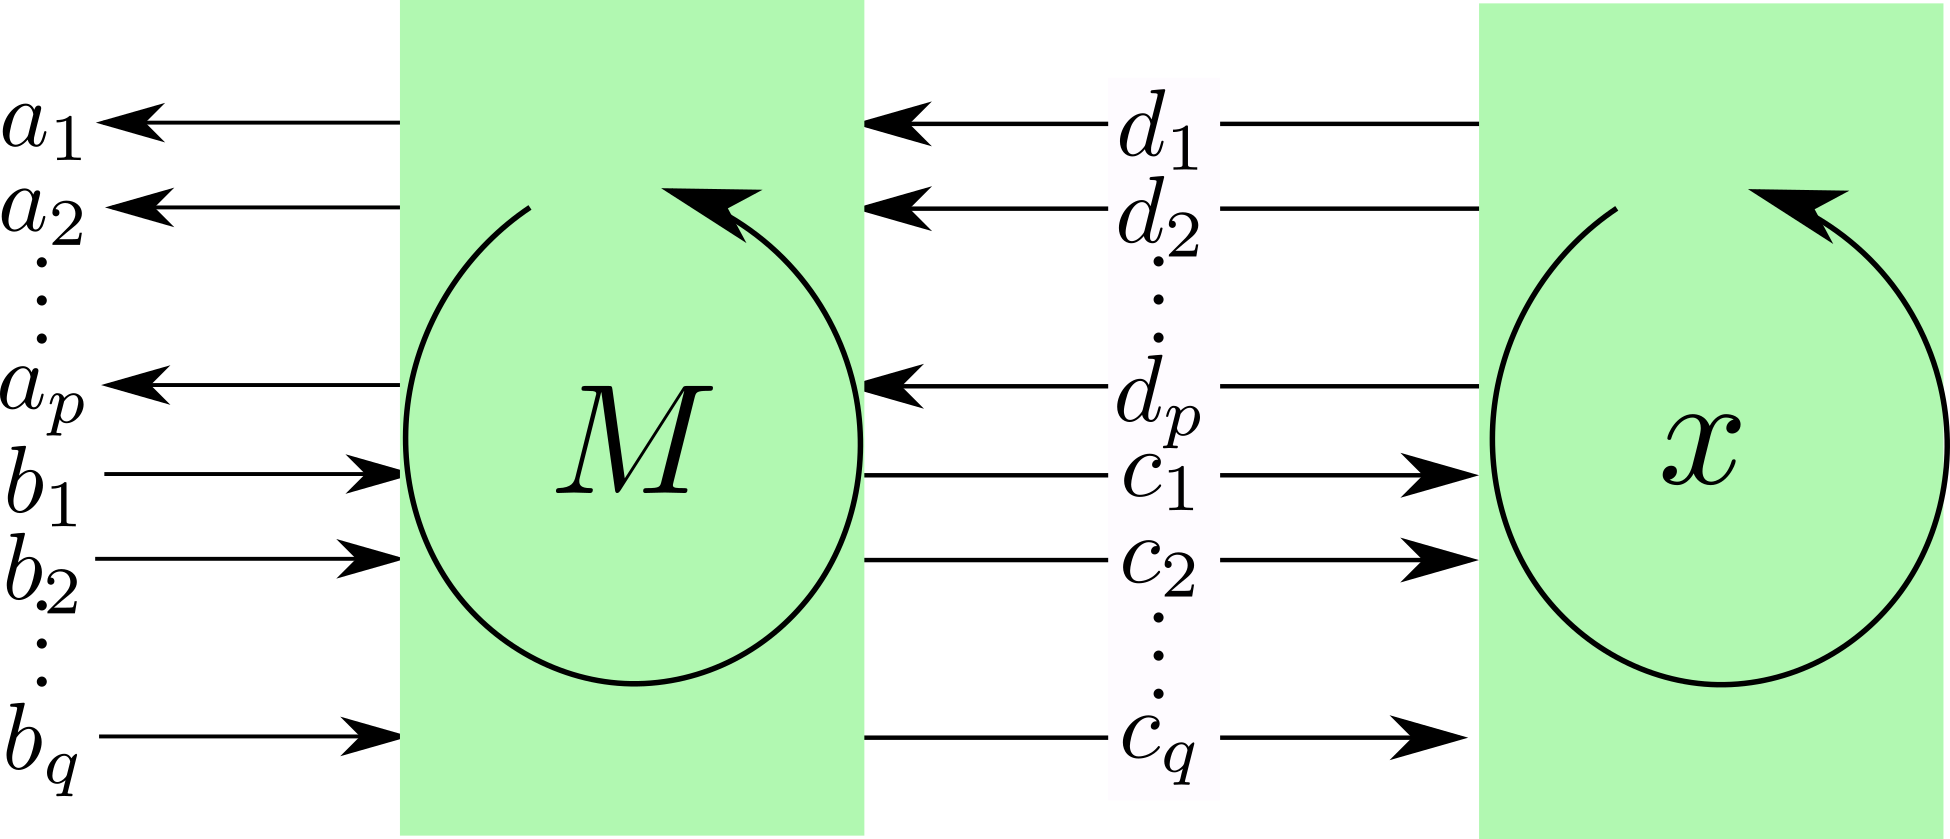
\includegraphics[width=2.7in]
{conventions/index-labels-Mx.png}
\caption{Index labels for $Mx$
where $M
\in \CC^{n^{p+q}\times n^{p+q}}$ and
$x\in V^{n^p}\otimes \dual{V}^{n^q}$.
Note that we  list indices in counterclockwise (CC) direction, 
starting at the top.}
\label{fig-index-labels-Mx}
\end{figure}

\begin{figure}[h!]
\centering
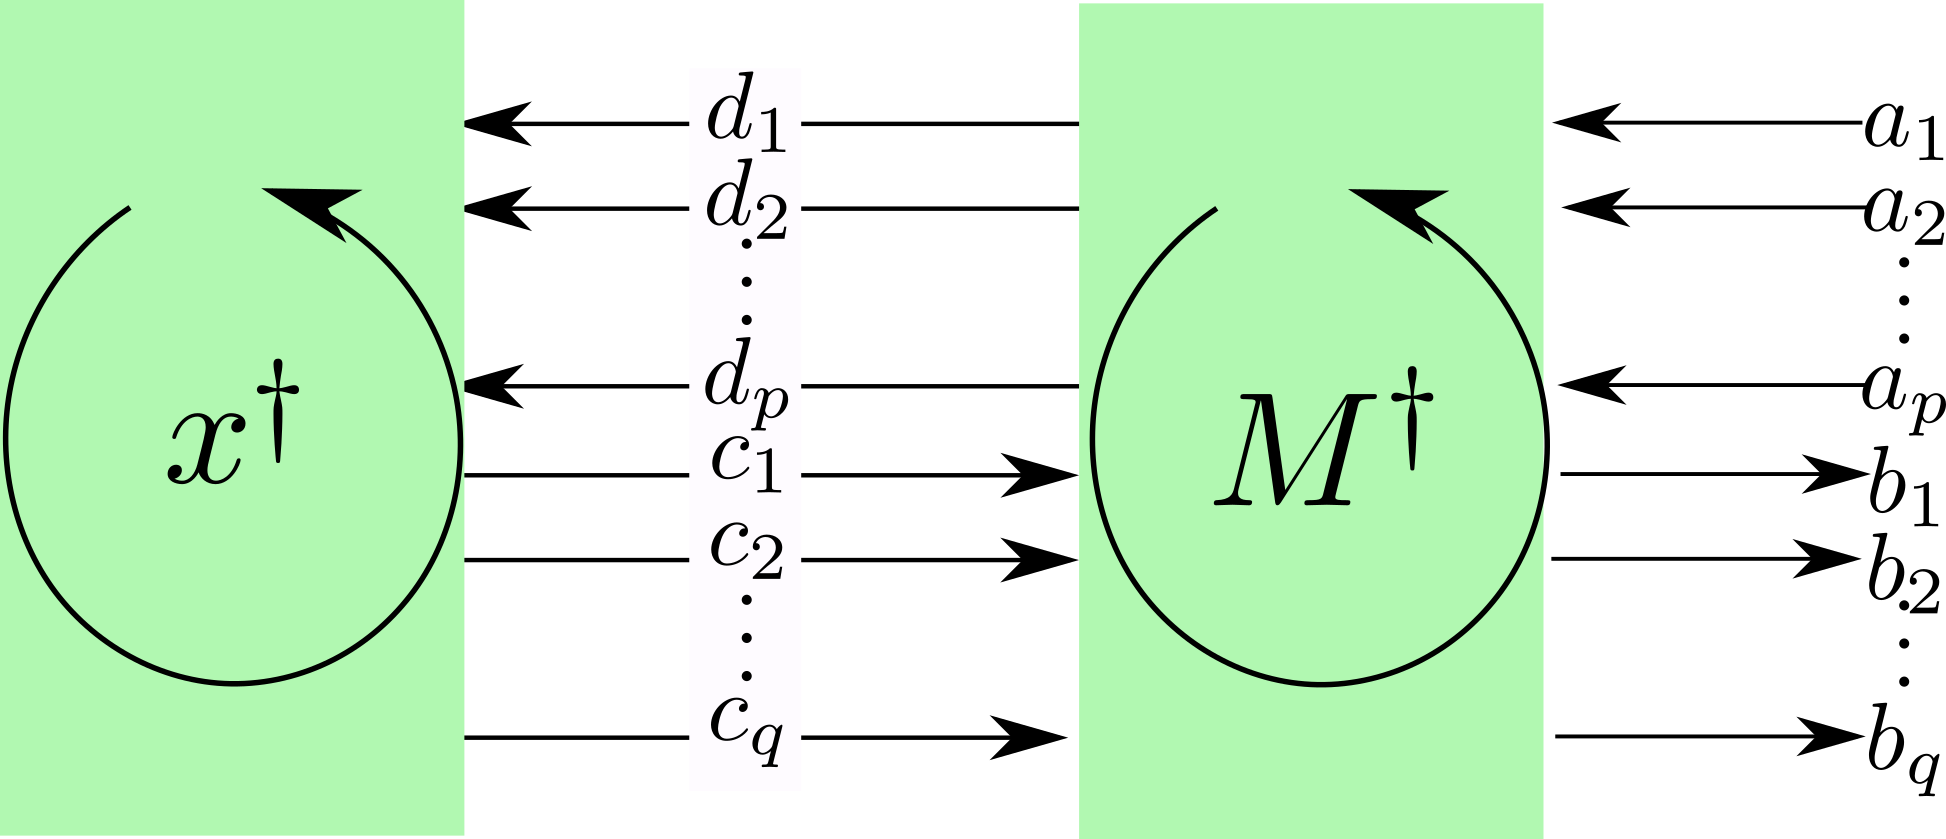
\includegraphics[width=2.7in]
{conventions/index-labels-hermitian.png}
\caption{Index labels for $x^\dagger M^\dagger$
corresponding to Fig.\ref{fig-index-labels-hermitian}.
Note that we  list indices in counterclockwise (CC) direction, 
starting at the top. }
\label{fig-index-labels-hermitian}
\end{figure}


Suppose $a_i, b_i, c_i, d_i\in \ZZ_{[1,n]}$.
From Fig.\ref{fig-index-labels-Mx}

\beq
y\indices{
_{a^{:p}}
^{b^{:q}}}=
M\indices{
_{a^{:p}}
^{b^{:q}}
_{rev(c^{:q})}
^{rev(d^{:p})}
}
x\indices{
_{d^{:p}}
^{c^{:q}}
}
\eeq
If we define $X_\alp$
and $x^\alp$ by

\beq
X\indices{_\alp} = X\indices{
_{a^{:p}}
^{b^{:q}}
}
,\quad
X\indices{^\alp}
=
X\indices{
_{rev(b^{:q})}
^{rev(a^{:p})}
}
\eeq
then

\beq
x_\alp = M\indices{_\alp^\beta}x_\beta
\eeq


\hrule

Hermitian conjugation (see Fig.\ref{fig-index-labels-hermitian})

\beq
\left\{
\begin{array}{l}
(M^\dagger)\indices{_a^d}=
(M\indices{_d^a})^*
\\
(M^\dagger)\indices{_\alp^{\delta}}=
(M\indices{
_{rev(\delta)}
^{rev(\alp)}
})^*
\end{array}\right.
\eeq
Note that
$\dagger$ does 3 things
to the birdtrack:

\begin{enumerate}
\item It flips the horizontal
axis of the figure. (In the
algebraic expression of the tensor, this
corresponds to
reversing the horizontal 
order of the indices.)

\item For each node, it changes incoming
arrows to outgoing ones and vice versa.
(In the
algebraic expression of the tensor, this
corresponds 
reversing the vertical
positions of the indices; i.e., 
lowering upper indices
and raising lower ones.)

\item
It replaces the tensor component
by its complex conjugate

\end{enumerate}


Hermitian matrix
 
\beq
M^\dagger
 = M,\quad
 \left\{
 \begin{array}{l}
(M\indices
{_d^a })^*
= M\indices{_a^d}
\\
(M\indices{_{rev(\delta)}^{rev(\alp)}})^*
=
M\indices{_\alp^{\delta}}
\end{array}
\right.
\eeq
Unitary matrix

\beq
M^\dagger
 M=1,\quad
 \left\{
 \begin{array}{l}
(M\indices
{_d^a })^*
M\indices{_a^d}=1
\\
(M\indices{_{rev(\delta)}^{rev(\alp)}})^*
M\indices{_\alp^{\delta}}=1
\end{array}
\right.
\eeq

\hrule

Note that
for $x\in V^n{}$, $y\in \dual{V}^n$, and $G\in \calg\subset GL(n, \CC)$,

\beq
(x')_a (y')^b= G\indices{^b_c} 
G\indices{_a^d}x_dy^c
\eeq


If $x\in V^{n^p}\otimes \dual{V}^{n^q}$, $\GG\in \calg\subset GL(n^{p+q}, \CC)$,

\beq
(x')\indices{
_{a^{:p}}
^{b^{:q}}
}
=
\GG\indices{
_{a^{:p}}
^{b^{:q}}
_{rev(c^{:q})}
^{rev(d^{:p})}
}
x\indices{
_{d^{:p}}
^{c^{:q}}
},
\quad
(x'_\alp=\GG\indices{_\alp^\beta}x_\beta)
\label{eq-xprime-eq-gg-x}
\eeq
where we define

\beq
\GG\indices{
_{a^{:p}}
^{b^{:q}}
_{rev(c^{:q})}
^{rev(d^{:p})}
}
\eqdef
\prod_{i=1}^p
G\indices{
_{a_i}
^{d_i}
}
\prod_{i=1}^q
\dual{G}\indices{
^{b_i}
_{c_i}
}
\eeq


\hrule
An issue that arises with tensors is this:
When is it permissible to represent 
a tensor by $M_{ab}^{cd}$?
If we define
$M_{ab}^{cd}$  by
\beq
M_{ab}^{cd} = M\indices{_a_b^c^d}
\eeq
then it's always permissible.
Then one can define
tensors like
$M\indices{_a^b^c^d}$
as 

\beq
M\indices{_a^b^c^d}=
g^{bb'}M\indices{_a_{b'}^c^d}
=
g^{bb'}M_{ab'}^{cd}
\eeq
Hence, one drawback of
using the notation
$M_{ab}^{cd}$
is that if one is interested 
in using versions of
$M_{ab}^{cd}$ with
some indices raised or 
lowered, one has to 
write down explicitly the metric tensors 
that do the lowering and
raising.
Instead of writing
$M\indices{_a^b^c^d}$,
you'll have to write
$g^{bb'}M_{ab'}^{cd}$.
This is not very onerous when 
explaining a topic
in which not much
lowering and raising of indices is
done. But in topics like
General Relativity that do
use a lot of raising and lowering of indices, it might not be 
too succinct.

\section{Permutations}
\label{sec-permutation-group}
Some well known notation 
and results about permutations are these.

$(1,2)$ stands for a {\bf transposition}; i.e., a map that swaps 1 and 2:


\beq\left(
\bcen
\footnotesize
\xymatrix@R=1pc@C=1pc{
1\ar[rd]
&2\ar[ld]
&3\ar[d]
&\ldots
&p\ar[d]
\\
1
&2
&3
&\ldots
&p
}
\ecen
\right)
\eeq

$(3,2,1)$ stands for a {\bf permutation}; i.e., a map that maps $3\rarrow 2\rarrow 1\rarrow 3$. 
\beq\left(
\bcen
\footnotesize
\xymatrix@R=1pc@C=1pc{
1\ar[rrd]
&2\ar[ld]
&3\ar[ld]
&4\ar[d]
&\ldots
&p\ar[d]
\\
1
&2
&3
&4
&\ldots
&p
}
\ecen
\right)
\eeq



Any
reordering of $(1,2,3,\ldots, p)$
is a permutation of $p$ letters (or numbers or elements).

The set $S_p$ of all permutation of
$p$ letters 
is called the {\bf symmetric group in $p$ letters}. It has $p!$ elements  (i.e., $|S_p|=p!$) and is a group,
where the group's product is map composition
and the group's identity element
is the identity map.

Any permutation can be expressed as a product of transpositions, For example,  $(3,2,1)=(3,2)(2,1)$.




An {\bf even permutation} such as
$(3,2,1)$ can be expressed as a product of an even number of 
transpositions. An {\bf odd permutation} can be expressed as a product of an odd
number of transpositions.